\section{Introduction}
\label{sec:intro}

Quantum machine learning (QML) offers models with no obvious classical
analogue, such as kernels defined by quantum feature
maps~\citep{huang2021power} and classifiers defined by measurements on quantum
states~\citep{hausladen1994pgm}. They are commonly evaluated by inserting one
into a strong classical pipeline and reporting the change in accuracy. In
continual learning these changes are often a few tenths of a point, about the
size of the pipeline's own run-to-run variation, and the classical alternative
to the quantum component is rarely tested~\citep{bowles2024better}. A recent
quantum method for class-incremental learning, for instance, reports single
numbers without variance~\citep{li2026qkd}.

We ask whether quantum components help \emph{exemplar-free class-incremental
learning} (CIL): a model learns new classes task after task, may not store
images of past tasks, and must classify all classes seen so far. The setting
suits quantum models for two reasons. The model must keep compact summaries of
past classes, and a density matrix is such a summary. Its main difficulty,
confusion between classes learned at different times, is a state-discrimination
problem. We start from RSIAT~\citep{rsiat}, a strong pre-trained baseline that
already stores one mean and one covariance per class.

Before testing any component we measured how much the baseline varies, and
built a protocol that resolves changes of $0.2$ points
(Section~\ref{sec:setup}). It pairs seeds and replicates, evaluates every
inference head on the same network, fixes decision rules before each run, and
gives every quantum component a \emph{classical twin} that receives the same
inputs. The first of these checks already overturned an earlier result of ours:
a $+0.36$ gain of a quantum-kernel variant over a single baseline run shrank to
$+0.06$ ($[-0.07,+0.18]$) under the protocol.

We then test quantum components wherever they can enter the pipeline
(Figure~\ref{fig:pipeline}). During training, a projected quantum kernel (PQK)
steers the base task or separates new features from old classes, and two
density-matrix objectives, the Holevo quantity and a measurement-based loss,
shape the adapter. At inference, the PQK serves as a feature map, and a
pretty-good measurement (PGM) over class density matrices classifies alone or
fused with the baseline classifier. Our contributions are:
\begin{itemize}
  \item \textbf{A measurement protocol} for small effects in CIL, and its
    application to seven quantum placements, each against its classical twin
    (Table~\ref{tab:quantum}). Only one twin comparison has an interval
    above zero, the PQK against the same circuit without entanglement, at $+0.04$ points of
    average accuracy; the PQK feature map loses up to $17$ points.
  \item \textbf{A diagnosis-then-repair study} of the quantum separation
    regulariser. A read-only probe locates its weaknesses (an 8-qubit
    projection that discards class information, saturated angles, a frozen
    kernel); repairing them makes average accuracy worse ($-0.07$, $[-0.11,-0.03]$).
  \item \textbf{Theory} explaining the measurement results: circuits applied
    after the encoding and the usual state shrinkage cannot change the PGM, so
    only the encoding remains as a quantum degree of freedom.
  \item \textbf{An analysis across 61 stored runs} showing that every
    training-time intervention we tried, quantum or not, trades accuracy on
    new tasks for accuracy on old tasks, and that only an inference-time fusion
    raises both. That fusion, with a classical or a quantum score, raises final
    accuracy on four benchmarks by $+0.38$ to $+0.67$ points.
\end{itemize}

\begin{figure*}[t]
\centering
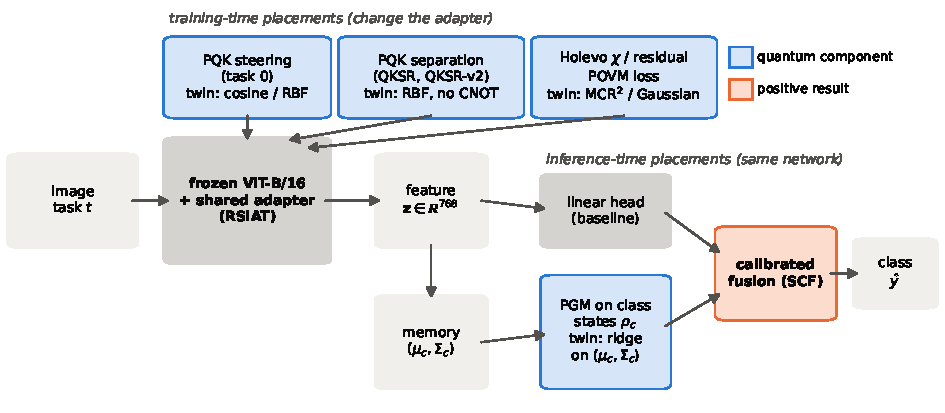
\includegraphics[width=0.92\textwidth]{figures/pipeline.pdf}
\caption{Where quantum components enter the RSIAT pipeline. Blue: quantum
placements, each listed with its classical twin. Training-time placements
change the shared adapter; inference-time placements are evaluated on the
same trained network. Orange: the calibrated score fusion (SCF), the only
component that raised both old- and new-task accuracy.}
\label{fig:pipeline}
\end{figure*}
